\cmfnewsection{Circuitos Simples para Aprender Usar Outros Blocos}{./logos/fundo_tese}{0.15}








%%%%%%%%%%%%%%%%%%%%%%%%%%%%%%%%%%%%%%%%%%%%%%%%
%%%%%%%%%%%%%%%%%%%%%%%%%%%%%%%%%%%%%%%%%%%%%%%%
%%%%%%%%%%%%%%%%%%%%%%%%%%%%%%%%%%%%%%%%%%%%%%%%
%%%%%%%%%%%%%%%%%%%%%%%%%%%%%%%%%%%%%%%%%%%%%%%%
\begin{frame}{Circuito 2A}
\centering



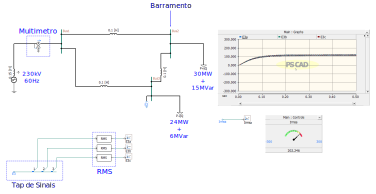
\includegraphics[width=0.95\linewidth]{./figuras/Segundo-Circuito/SIM2a}



\end{frame}






%%%%%%%%%%%%%%%%%%%%%%%%%%%%%%%%%%%%%%%%%%%%%%%%
%%%%%%%%%%%%%%%%%%%%%%%%%%%%%%%%%%%%%%%%%%%%%%%%
%%%%%%%%%%%%%%%%%%%%%%%%%%%%%%%%%%%%%%%%%%%%%%%%
%%%%%%%%%%%%%%%%%%%%%%%%%%%%%%%%%%%%%%%%%%%%%%%%
\begin{frame}{Circuito 2B}
\centering



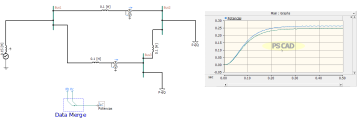
\includegraphics[width=0.95\linewidth]{./figuras/Segundo-Circuito/SIM2b}



\end{frame}







%%%%%%%%%%%%%%%%%%%%%%%%%%%%%%%%%%%%%%%%%%%%%%%%
%%%%%%%%%%%%%%%%%%%%%%%%%%%%%%%%%%%%%%%%%%%%%%%%
%%%%%%%%%%%%%%%%%%%%%%%%%%%%%%%%%%%%%%%%%%%%%%%%
%%%%%%%%%%%%%%%%%%%%%%%%%%%%%%%%%%%%%%%%%%%%%%%%
\begin{frame}{Circuito 2C}
\centering



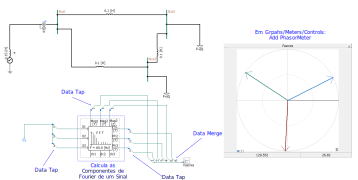
\includegraphics[width=0.95\linewidth]{./figuras/Segundo-Circuito/SIM2c}



\end{frame}







%%%%%%%%%%%%%%%%%%%%%%%%%%%%%%%%%%%%%%%%%%%%%%%%
%%%%%%%%%%%%%%%%%%%%%%%%%%%%%%%%%%%%%%%%%%%%%%%%
%%%%%%%%%%%%%%%%%%%%%%%%%%%%%%%%%%%%%%%%%%%%%%%%
%%%%%%%%%%%%%%%%%%%%%%%%%%%%%%%%%%%%%%%%%%%%%%%%
\begin{frame}{Circuito 2D: Nosso primeiro circuito monofásico}
\centering



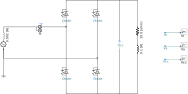
\includegraphics[width=0.75\linewidth]{./figuras/Segundo-Circuito/SIM2d}



\end{frame}






%%%%%%%%%%%%%%%%%%%%%%%%%%%%%%%%%%%%%%%%%%%%%%%%
%%%%%%%%%%%%%%%%%%%%%%%%%%%%%%%%%%%%%%%%%%%%%%%%
%%%%%%%%%%%%%%%%%%%%%%%%%%%%%%%%%%%%%%%%%%%%%%%%
%%%%%%%%%%%%%%%%%%%%%%%%%%%%%%%%%%%%%%%%%%%%%%%%
\begin{frame}{Circuito 2D: FFT}
\centering


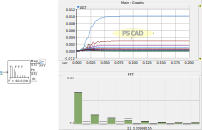
\includegraphics[width=0.70\linewidth]{./figuras/Segundo-Circuito/SIM2d-FFT}

\end{frame}




%%%%%%%%%%%%%%%%%%%%%%%%%%%%%%%%%%%%%%%%%%%%%%%%
%%%%%%%%%%%%%%%%%%%%%%%%%%%%%%%%%%%%%%%%%%%%%%%%
%%%%%%%%%%%%%%%%%%%%%%%%%%%%%%%%%%%%%%%%%%%%%%%%
%%%%%%%%%%%%%%%%%%%%%%%%%%%%%%%%%%%%%%%%%%%%%%%%
\begin{frame}{Circuito 2E: Transformadores e etc}
\centering


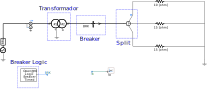
\includegraphics[width=0.70\linewidth]{./figuras/Segundo-Circuito/SIM2e}

\end{frame}






%%%%%%%%%%%%%%%%%%%%%%%%%%%%%%%%%%%%%%%%%%%%%%%%
%%%%%%%%%%%%%%%%%%%%%%%%%%%%%%%%%%%%%%%%%%%%%%%%
%%%%%%%%%%%%%%%%%%%%%%%%%%%%%%%%%%%%%%%%%%%%%%%%
%%%%%%%%%%%%%%%%%%%%%%%%%%%%%%%%%%%%%%%%%%%%%%%%
\begin{frame}{Circuito 2F: Máquinas CC}
\centering


\begin{columns}

\column{0.4\linewidth}
\centering
Máquina
\vspace*{0.5cm}

\includegraphics[width=0.95\linewidth]{./figuras/Segundo-Circuito/maquina_CC_b}

\column{0.6\linewidth}
\centering
Modelo Matemático\footnote[frame]{\tiny Stephen J. Chapman, Fundamentos das Máquinas Elétricas. 5ed. Capítulos 7 e 8.}
\vspace*{1cm}

\includegraphics[width=0.95\linewidth]{./figuras/Segundo-Circuito/SIMf_dc_machine}

\end{columns}

\end{frame}





%%%%%%%%%%%%%%%%%%%%%%%%%%%%%%%%%%%%%%%%%%%%%%%%
%%%%%%%%%%%%%%%%%%%%%%%%%%%%%%%%%%%%%%%%%%%%%%%%
%%%%%%%%%%%%%%%%%%%%%%%%%%%%%%%%%%%%%%%%%%%%%%%%
%%%%%%%%%%%%%%%%%%%%%%%%%%%%%%%%%%%%%%%%%%%%%%%%
\begin{frame}{Circuito 2F: Mais Sobre o Modelo da Máquina}
\centering


\begin{columns}



\column{0.25\linewidth}
\centering

{\color{blue}Movimento

+

Fluxo  Magnético

$\downarrow$ 

Tensão Induzida
}





\column{0.5\linewidth}
\centering


\includegraphics[width=0.85\linewidth]{./figuras/Segundo-Circuito/SIMf_dc_machine_excitation}




\column{0.25\linewidth}
\centering

{\color{blue}Corrente

+

Fluxo  Magnético

$\downarrow$ 

Torque
}

\end{columns}
\end{frame}




%%%%%%%%%%%%%%%%%%%%%%%%%%%%%%%%%%%%%%%%%%%%%%%%
%%%%%%%%%%%%%%%%%%%%%%%%%%%%%%%%%%%%%%%%%%%%%%%%
%%%%%%%%%%%%%%%%%%%%%%%%%%%%%%%%%%%%%%%%%%%%%%%%
%%%%%%%%%%%%%%%%%%%%%%%%%%%%%%%%%%%%%%%%%%%%%%%%
\begin{frame}{Circuito 2F: Máquinas CC no PSCAD}
\centering


\begin{columns}

\column{0.4\linewidth}
\centering

\begin{itemize}
\item Representa apenas as equações elétricas 
\vspace*{2cm}
\item A dinâmica mecânica é deixada de lado
\end{itemize}

\column{0.6\linewidth}
\centering


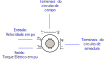
\includegraphics[width=0.95\linewidth]{./figuras/Segundo-Circuito/SEMf_maq_cc_pascad}

\end{columns}
\end{frame}




%%%%%%%%%%%%%%%%%%%%%%%%%%%%%%%%%%%%%%%%%%%%%%%%
%%%%%%%%%%%%%%%%%%%%%%%%%%%%%%%%%%%%%%%%%%%%%%%%
%%%%%%%%%%%%%%%%%%%%%%%%%%%%%%%%%%%%%%%%%%%%%%%%
%%%%%%%%%%%%%%%%%%%%%%%%%%%%%%%%%%%%%%%%%%%%%%%%
\begin{frame}{Circuito 2F: Modelando a Dinâmica Mecânica}
\centering


\begin{columns}

\column{0.5\linewidth}

{\it Lei de Newton} dos sistemas rotacionais:
\begin{equation*}
J \frac{d \omega_m}{dt} = T_e - T_m 
\end{equation*}



\column{0.5\linewidth}

Convertendo para pu: 
\begin{equation*}
2 H \frac{d \omega_{m,pu}}{dt}  = T_{e,pu} - T_{m,pu} 
\end{equation*}




\end{columns}

\begin{equation*}
H = \frac{J}{2}  \frac{\omega_{nominal}}{P_{nominal}}
\end{equation*}

\begin{itemize}
\item $T_e$ - Torque eletromagnético (calculado pelo modelo da máquina)
\item $T_m$ - Torque mecânico 
\item $\omega_m$ - Velocidade mecânica
\end{itemize}

\end{frame}







%%%%%%%%%%%%%%%%%%%%%%%%%%%%%%%%%%%%%%%%%%%%%%%%
%%%%%%%%%%%%%%%%%%%%%%%%%%%%%%%%%%%%%%%%%%%%%%%%
%%%%%%%%%%%%%%%%%%%%%%%%%%%%%%%%%%%%%%%%%%%%%%%%
%%%%%%%%%%%%%%%%%%%%%%%%%%%%%%%%%%%%%%%%%%%%%%%%
\begin{frame}{Circuito 2F: Circuito}
\centering

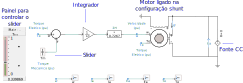
\includegraphics[width=0.9\linewidth]{./figuras/Segundo-Circuito/SIM2f}

\end{frame}